% 惠斯登电桥

\pentry{电阻\upref{Resist}}

% 未完成: 改成图 2 的矢量图
\begin{figure}[ht]
\centering
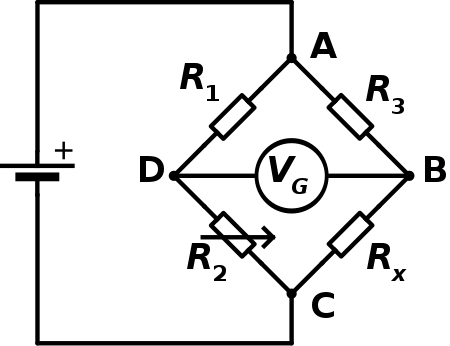
\includegraphics[width=5cm]{./figures/WheBrg_1.png}
\caption{惠斯登电桥} \label{WheBrg_fig1}
\end{figure}

求惠斯通(Wheatstone)电桥\autoref{WheBrg_fig2}中电流计的电流$I_G$与电源电动势及各臂电阻的关系(电源内阻可忽略).
\begin{figure}[ht]
\centering
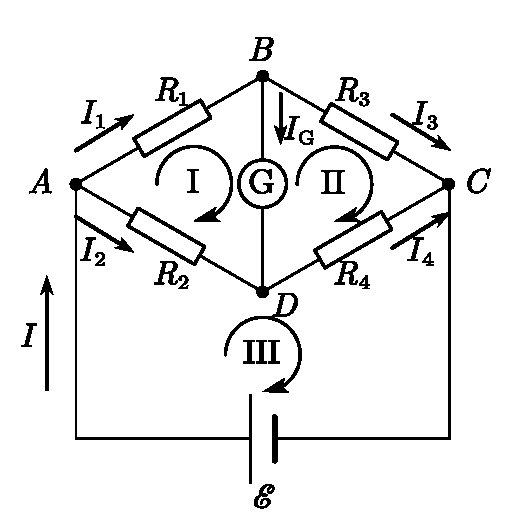
\includegraphics[width=6cm]{./figures/WheBrg_2.pdf}
\caption{惠斯通电桥} \label{WheBrg_fig2}
\end{figure}

选定各支路电流$I_{1}, I_{2}, I_{3}, I_{4}, I_{\mathrm{G}}$及$I $的正方向如\autoref{WheBrg_fig2}中实箭头
所示.因节点数$n = 4$,故可列出三个节点方程:
\begin{equation}
\begin{array}{ll}\text { 节点 } A: & I=I_{1}+I_{2} \\ \text { 节点 } B: & I_{1}=I_{3}+I_{G} \\ \text { 节点 } C: & I_{3}+I_{4}=I\end{array}
\end{equation}
又因支路数$b=6$,故独立回路数$m=b-n+1=3$选图中$\rm I$、$\rm II$、$\rm III$三个独立回路,约定其绕行方向如图圆形箭头所示,列出回路方程:
\begin{equation}
\begin{array}{ll}\text { 回路 } \mathrm{I}: & I_{1} R_{1}+I_{\mathrm{G}} R_{\mathrm{G}}-I_{2} R_{2}=0 \\ \text { 回路 } \mathrm{II}: & I_{3} R_{3}-I_{4} R_{4}-I_{\mathrm{G}} R_{\mathrm{G}}=0 \\ \text { 回路 } \mathrm{II}  : & I_{2} R_{2}+I_{4} R_{4}=\mathscr{E}\end{array}
\end{equation}
六个方程联立解得:
\begin{equation} \label{WheBrg_eq6}
I_{\mathrm{G}}=\frac{\left(R_{2} R_{3}-R_{1} R_{4}\right) \mathscr{E}}{{R}_{1} R_{3}\left(R_{2}+R_{4}\right)+R_{2} R_{4}\left(R_{1}+R_{3}\right)+R_{\mathrm{G}}\left(R_{1}+R_{3}\right)\left(R_{2}+R_{4}\right)}
\end{equation}
由上式可知电桥平衡(即$I_\mathrm{G} = 0$)的充要条件为
\begin{equation}
R_{1} R_{4}=R_{2} R_{3}
\end{equation}
\autoref{WheBrg_eq6}说明,当$R_{2} R_{3}-R_{1} R_{4}>0$时$I_{\mathrm{G}}>0$,电流$I_{\mathrm{G}}$的实际方向与正方向一致(向下);反之,当$R_{2} R_{3}-R_{1} R_{4}<0$时$I_{\mathrm{G}}<0$,$I_{\mathrm{G}}$的实际方向与正方向相反(向上).
